\documentclass{beamer}
%\documentclass[handout]{beamer}

\mode<presentation>
{
  \usetheme{CambridgeUS}
  \usefonttheme{professionalfonts}
  \usefonttheme[onlymath]{serif}
}

\usepackage{pgfpages}

\usepackage{alltt,verbatim,amsmath,times}
\usepackage{bm}
\usepackage[english]{babel}
\usepackage[utf8]{inputenc}

%\usepackage{times}
%\usepackage[T1]{fontenc}
% Or whatever. Note that the encoding and the font should match. If T1
% does not look nice, try deleting the line with the fontenc.

\usepackage{hyperref}

\newcommand{\CC}{\mathbb{C}}
\newcommand{\NN}{\mathbb{N}}
\newcommand{\RR}{\mathbb{R}}
\newcommand{\ZZ}{\mathbb{Z}}
\newcommand{\Acal}{\mathcal{A}}
\newcommand{\Bcal}{\mathcal{B}}
\newcommand{\Ccal}{\mathcal{C}}
\newcommand{\Ncal}{\mathcal{N}}
\newcommand{\Kcal}{\mathcal{K}}

\newcommand{\bF}{\mathbf{F}}
\newcommand{\bQ}{\mathbf{Q}}
\newcommand{\bU}{\mathbf{U}}
\newcommand{\bbU}{\bar{\bU}}
\newcommand{\bu}{\mathbf{u}}
\newcommand{\bv}{\mathbf{v}}
\newcommand{\bx}{\mathbf{x}}

\newcommand{\Div}{\nabla\cdot}
\newcommand{\eps}{\epsilon}
\newcommand{\grad}{\nabla}
\newcommand{\lap}{\triangle}
\DeclareMathOperator{\trace}{tr}
\renewcommand{\bar}{\overline}

\newcommand{\ddx}[1]{\frac{\partial #1}{\partial x}}
\newcommand{\ddy}[1]{\frac{\partial #1}{\partial y}}
\newcommand{\pp}[2]{\frac{\partial #1}{\partial #2}}
\newcommand{\ppt}[1]{\frac{\partial #1}{\partial t}}
\newcommand{\ppT}[1]{\frac{\partial #1}{\partial T}}
\newcommand{\ppx}[1]{\frac{\partial #1}{\partial x}}
\newcommand{\ppy}[1]{\frac{\partial #1}{\partial y}}
\newcommand{\ppz}[1]{\frac{\partial #1}{\partial z}}
\newcommand{\ppxx}[1]{\frac{\partial^2 #1}{\partial x^2}}
\newcommand{\ppzz}[1]{\frac{\partial^2 #1}{\partial z^2}}

%\setbeamercolor{redtext}{fg=red!80!black}
\setbeamercolor{redtext}{fg=red!94!black}
%\setbeamercolor{greentext}{fg=green!80!black}
\setbeamercolor{greentext}{fg=green!60!black}
%\setbeamercolor{bluetext}{fg=blue!70!black}
\setbeamercolor{bluetext}{fg=blue!90!black}
\setbeamercolor{yellowtext}{fg=yellow!95!black}
\setbeamercolor{orangetext}{fg=yellow!50!red}

\newcommand{\green}{\usebeamercolor[fg]{greentext}}
\newcommand{\blue}{\usebeamercolor[fg]{bluetext}}
\newcommand{\red}{\usebeamercolor[fg]{redtext}}

\renewcommand{\L}{\emph{Left}}
\newcommand{\R}{\emph{Right}}



\title[weak and shallow ice sheet flow]{Weak and shallow: \\ New thinking on simulations of ice sheet flows}

\author[Bueler]{Ed Bueler}

\institute[UAF]{
  \tiny Dept of Mathematics and Statistics, and Geophysical Institute,
  University of Alaska Fairbanks
}

\date{\tiny 27 October, 2012}


\setbeamerfont{date}{size=\scriptsize}

\subject{ice sheet modelling, ice sheets, ice streams, numerical analysis, variational inequality}


%\begin{comment}
\AtBeginSection[]
{
  \begin{frame}<beamer>
    \frametitle{Outline}
    \tableofcontents[currentsection]
  \end{frame}
}
%\end{comment}


\begin{document}
\graphicspath{{figs/},{../commonfigs/}}

\begin{frame}
  \titlepage
  \begin{center}
  \tiny supported by NASA grant NNX09AJ38C
  \end{center}
\end{frame}

% NO OUTLINE BECAUSE ONE APPEARS AT START OF EACH SECTION:
\begin{comment}
\begin{frame}
  \frametitle{Outline}
  \tableofcontents[hideallsubsections]
  % You might wish to add the option [pausesections]
\end{frame}
\end{comment}


\section[intro]{ice sheets: an introduction}


\begin{frame}
  \frametitle{ice sheet flow affects sea level}

\small
\begin{itemize}
\item \emph{inputs}: (1) snow adds, (2) sun heats, (3) earth heats
\item \emph{outputs}: (1) surface meltwater, (2) basal meltwater, (3) ice discharge
\end{itemize}

\begin{center}
  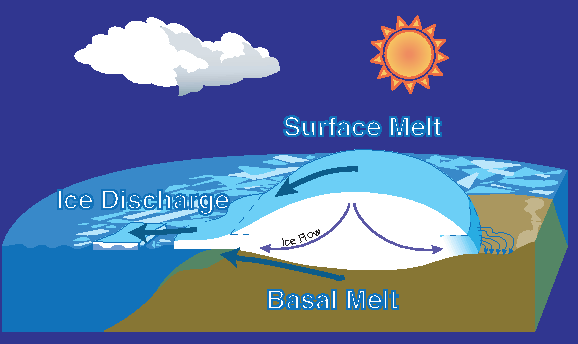
\includegraphics[width=0.7\textwidth]{ice-sheet-cartoon}

  \tiny (figure from IceSAT brochure)
\end{center}
\end{frame}


\begin{frame}
  \frametitle{ice sheet flow changes over time}

\small
\begin{itemize}
\item Greenland ice sheet mass is $2.7 \times 10^9$ gigatonnes (Gt) % = 2.93466 10^6 km^3  volume, from SeaRISE-Greenland 5km data
\item if \emph{all} ice melts then we get 7 m of sea level rise
\end{itemize}

\begin{center}
    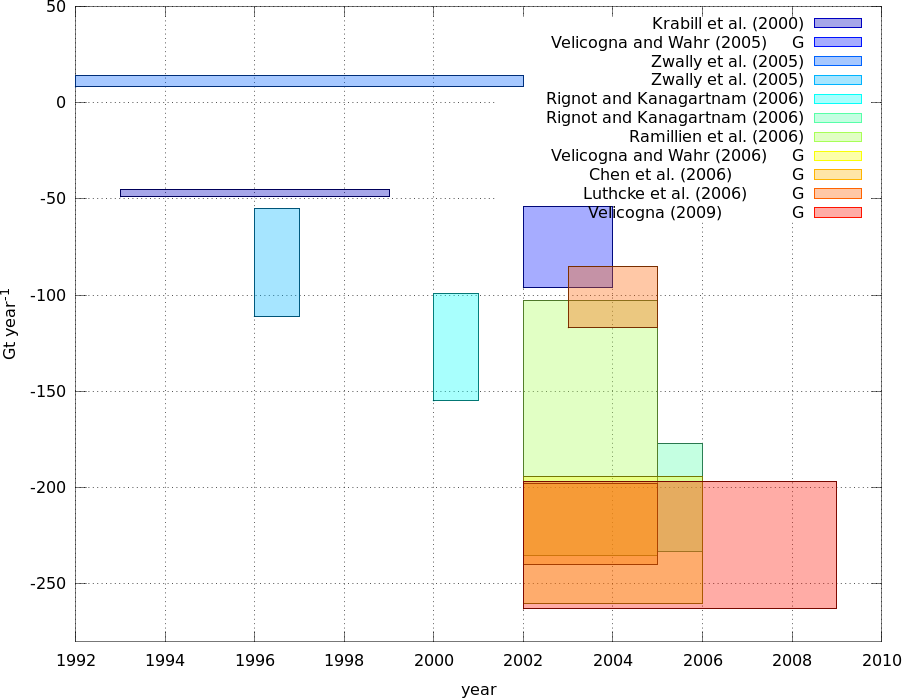
\includegraphics[width=0.7\textwidth]{greenlandboxes}
\end{center}
\end{frame}


\begin{frame}
  \frametitle{ice sheet flow varies in space}

\small
\begin{itemize}
\item csurf from PISM
\item cbase from PISM
\item FIXME: dh/dt for greenland from some source
\end{itemize}

\end{frame}


\section[shallow ice approximation]{the shallow ice sheet approximation}


\begin{frame}
  \frametitle{a shallow ice approximation (SIA) analogy}

\begin{columns}
\begin{column}{0.35\textwidth}
\begin{itemize}
\item ice sheet surface \\ = \alert{membrane}
\item bedrock = \alert{obstacle}
\end{itemize}

\vfill
\begin{center}
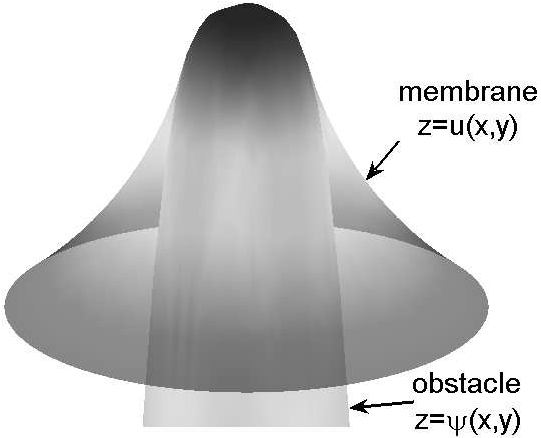
\includegraphics[width=1.1\textwidth]{classicalobs}
\end{center}
\end{column}

\begin{column}{0.65\textwidth}
\begin{center}
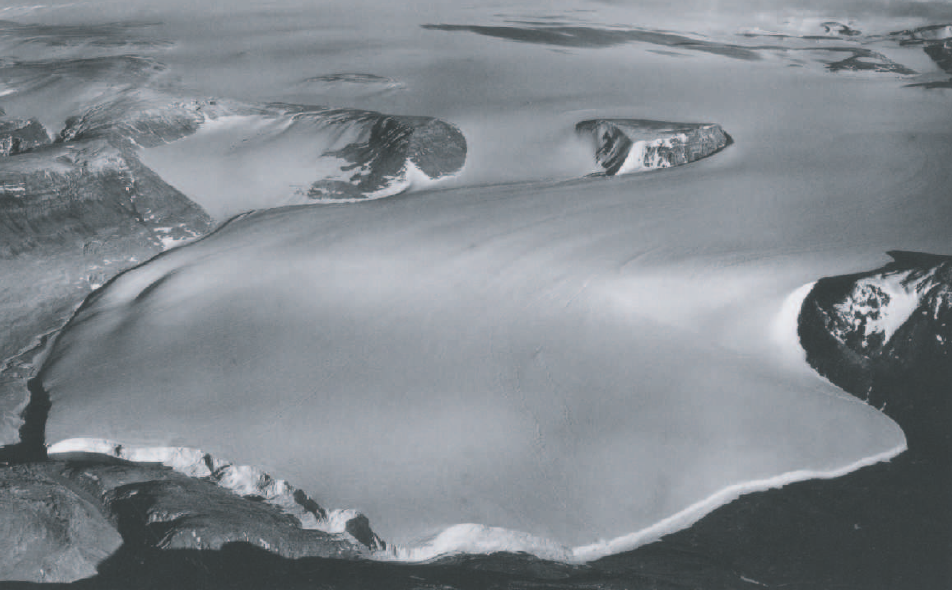
\includegraphics[width=0.8\textwidth]{polaris} \\
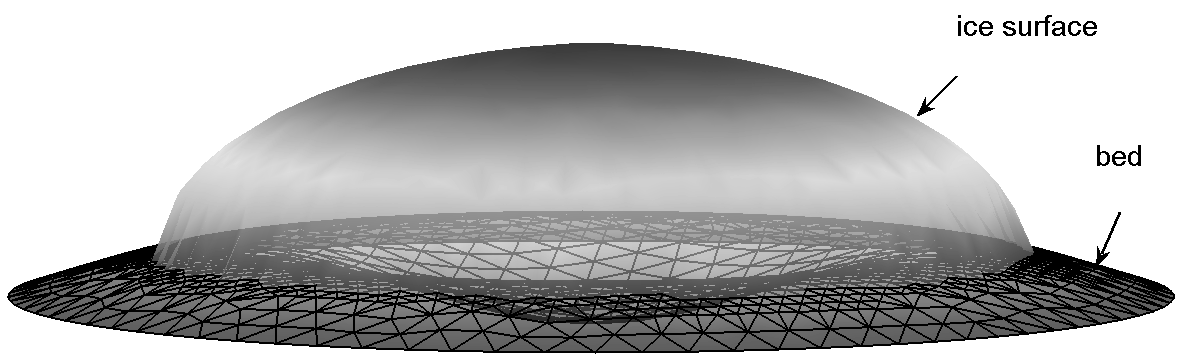
\includegraphics[width=\textwidth]{capnonflatobs}
\end{center}
\end{column}

\end{columns}
\end{frame}


\begin{frame}
  \frametitle{physical variables}

\begin{center}
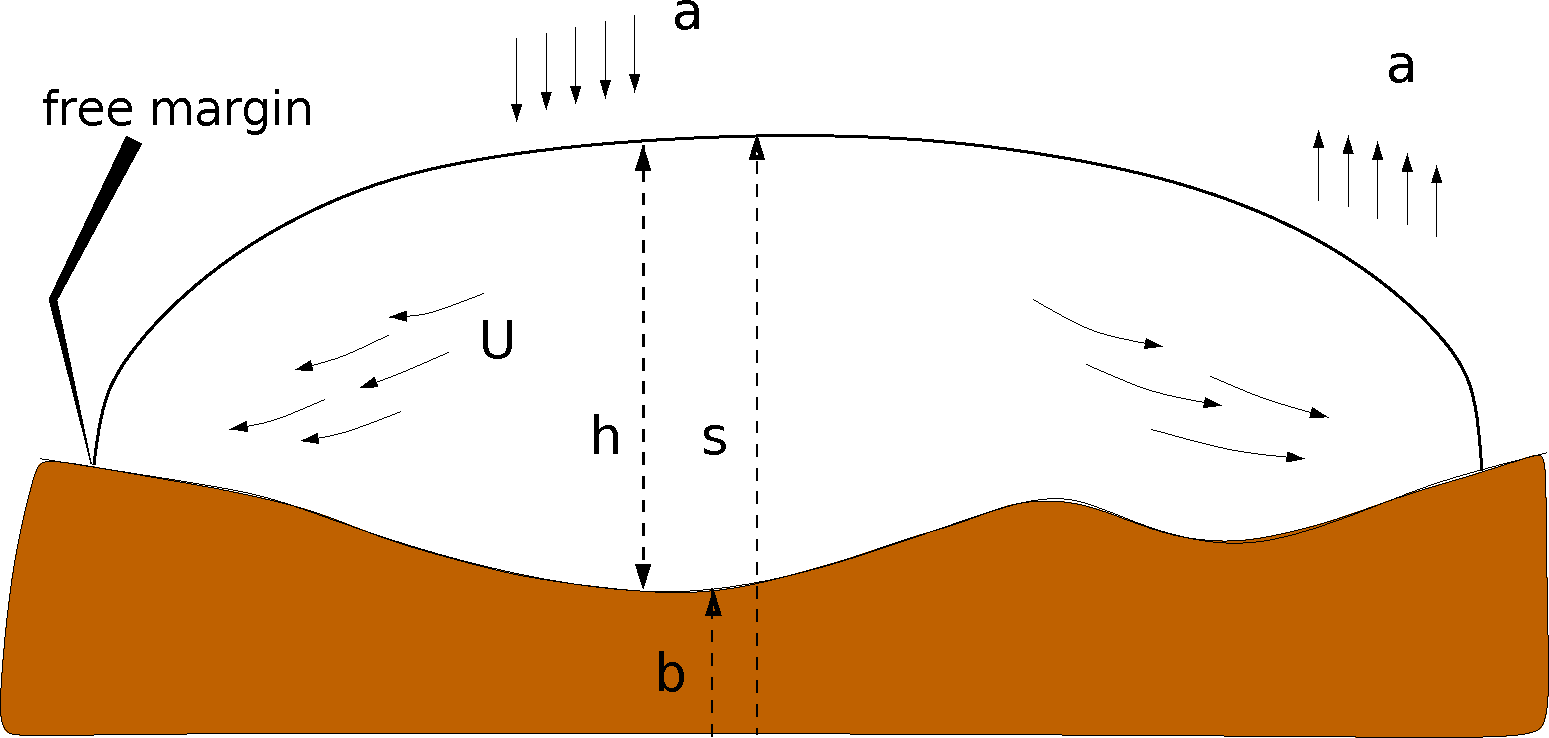
\includegraphics[width=0.7\textwidth]{groundedscheme}
\end{center}

\begin{itemize}
\item $b=b(\bx)$ the bedrock
\item $s=s(\bx,t)$ the top surface elevation
\item $h=h(\bx,t)$ the ice thickness
\item ${\bf U}={\bf U}(\bx,z)$ the horizontal velocity field
\item $a=a(\bx,z)$ the yearly-average mass balance
\end{itemize}
\end{frame}


\frame{  \frametitle{ Full and simplified ice flow models }

\onslide<+-> 

Ice is considered as a non-Newtonian incompressible fluid. \\
\hfill $\Rightarrow$ non-linear Stokes equations.

\onslide<+-> 
 
\begin{center}
\begin{tabular}{|c|c|c|c|}
\hline Order & Name & Unknowns  & Equation (+Incompressibility)   \\ 
\hline $\infty$-th &  Stokes & 
$\left(
\begin{array}{c}
u \\ 
v \\ 
w  
\end{array} \right),p$ &  
$  \nabla \cdot \left(
\begin{array}{ccc}
\tau_{xx} & \tau_{xy} & \tau_{xz} \\ 
\tau_{yx} & \tau_{yy} & \tau_{yz} \\ 
\tau_{zx} & \tau_{zy} & \tau_{zz}  
\end{array} \right) = \left(
\begin{array}{c}
0 \\ 
0 \\ 
\rho g  
\end{array} \right)$  \\ 
\hline $1$-th & FOA\footnote{First Order Approximation} & 
$\left(
\begin{array}{c}
u \\ 
v 
\end{array} \right) $  & 
$ \nabla \cdot \left(
\begin{array}{ccc}
\tau_{xx} & \tau_{xy} & \tau_{xz} \\ 
\tau_{yx} & \tau_{yy} & \tau_{yz} \\ 
0 & 0 & \tau_{zz}  
\end{array} \right) = \left(
\begin{array}{c}
0 \\ 
0 \\ 
\rho g  
\end{array} \right)$  \\  
\hline $0$-th & SSA\footnote{Shallow Shelf Approximation} &
$ \left(
\begin{array}{c}
u \\ 
v  
\end{array} \right) $ & 
$ \nabla \cdot \left(
\begin{array}{ccc}
\tau_{xx} & \tau_{xy} & 0 \\ 
\tau_{yx} & \tau_{yy} & 0 \\ 
0 & 0 & \tau_{zz}  
\end{array} \right) = \left(
\begin{array}{c}
0 \\ 
0 \\ 
\rho g  
\end{array} \right)$ \\ 
\hline $0$-th & SIA\footnote{Shallow Ice Approximation} & $\emptyset$ &
$ \nabla \cdot \left(
\begin{array}{ccc}
0 & 0 & \tau_{xz} \\ 
0 & 0 & \tau_{yz} \\ 
0 & 0 & \tau_{zz}  
\end{array} \right) = \left(
\begin{array}{c}
\rho g \frac{\partial s}{\partial x}\\ 
\rho g \frac{\partial s}{\partial y} \\ 
\rho g  
\end{array} \right)$ \\ 
\hline 
\end{tabular}  
\end{center}
  
}
  

\frame{  \frametitle{ The Shallow Ice Approximation / Mass conservation }
 
\onslide<+-> 
 
\begin{itemize}
\item Assuming no sliding and isothermal ice,  
ice velocity ${\bf U}$ is given  by: 
$$ {\bf U}(\bx,z)  =  - (2A/p) (\rho_i g)^{p-1}  \left[ (s-b)^p - (s - z)^p  \right] 
|\nabla s |^{p-2} \nabla s.$$ 

\onslide<+->

\item Mass conservation (in a steady state) writes: 
$\displaystyle \Div \left(  \int_b^s {\bf U} dz \right)  =  a. $

\end{itemize}  
  
\begin{center}
%\includegraphics[height=4cm]{fig/MC.pdf}
\begin{picture}(0,0)(0,0)
\put(-75,40){$ {\bf U} $} 
\put(-90,110){Mass balance $a$} 
\put(-105,85){$s$}  
\put(-110,15){$b$}  
\end{picture}    
\end{center}
 
}


\frame{  \frametitle{ Change of variable }
 
\onslide<+-> 

The Shallow Ice Approximation + Mass conservation:

$$ - \Gamma  \; {\rm div} \left( (s-b)^{p+1} | \nabla s |^{p-2} \nabla s  \right) =  a(s). $$
  
\onslide<+->   
  
Using the change of variable  $u=(s-b)^{ \frac{2p}{p-1}}$, we obtain:

\begin{equation*}
 -  \Div \left( \mu  | \nabla u - \Phi(u) |^{p-2} 
  ( \nabla u - \Phi(u) )  \right)  = \alpha(u), 
\end{equation*}   

\onslide<+-> 

where 
$$ \Phi(u) = - C \, u^{\frac{p+1}{2p}} \nabla b(\bx),
 \qquad \alpha(u) = a(\bx,u^{\frac{p-1}{2p}} )
\qquad {\rm and} \qquad \mu>0. $$
 
}


\frame{  \frametitle{ Variational inequality } 

\onslide<+-> 

In fact, we have:
 
\begin{align*}
 -  \Div \left( \mu  | \nabla u - \Phi(u) |^{p-2} 
  ( \nabla u - \Phi(u) )  \right) & = \alpha(u), & {\rm if} \; u > 0, \\
  u & = 0, & {\rm else.}
\end{align*}  

\onslide<+-> 

The change $u=(s-b)^{ \frac{2p}{p-1}}$ 
transforms the constrain $s \ge b$ into $u \ge 0$. 

\onslide<+-> 
    
\begin{block}{Definition} 
A function $u \in \Kcal := \{ v \in W^{1,p}_0 (\Omega), v \ge 0 \}$ 
solves the (transformed) steady shallow ice sheet problem if
\begin{align*}
\int_{\Omega}    \left( \mu  | \nabla u - \Phi(u) |^{p-2} 
( \nabla u - \Phi(u) )    \right)  \cdot \nabla ( v - u )  
\ge \int_{\Omega} \alpha(u) (  v -  u ) 
\end{align*}
for all $v \in \Kcal$.
\end{block}

}


\frame{  \frametitle{ Existence and uniqueness of solutions } 

 \onslide<+-> 

\begin{block}{Convex minimization}
If $a$ is independent of $u$, the variational inequality rewrites:
\begin{equation*}
J(u) = \min_{v \in \Kcal} \left\{  J(v):= \frac{\mu}{p} \int_{\Omega} 
 |\nabla v - \Phi |^p - \int_{\Omega}  \alpha v \right\} 
\end{equation*}
which admits a unique solution.
\end{block}

 \onslide<+->

\hfill $ \Rightarrow $ Existence and uniqueness only if the bedrock is flat ($\Phi = 0$). \\

 \onslide<+->
 
\begin{block}{Monotone operator}
If $a$ is not increasing with respect to $u$, 
we still have a unique solution by monotonicity of 
\begin{center}
$(Av)(w)= \mu \int_{\Omega} | \nabla v - \Phi|^{p-2} ( \nabla v  - \Phi )
\cdot \nabla w - \int_{\Omega}  \alpha(v) w .$
\end{center}
\end{block}
}
 
 
\frame{  \frametitle{ Existence in the general case } 

 \onslide<+->

Define the map $\mathcal{A}:C(\overline{\Omega}) \rightarrow C(\overline{\Omega})$,
which takes $w$ to the unique $u$ solving, for all $v \in \mathcal{K}$:
\begin{align*}
\int_{\Omega}   \mu  \left( | \nabla u - \Phi(w) |^{p-2} 
( \nabla u - \Phi(w) )    \right)  \cdot \nabla ( v - u )  
\ge \int_{\Omega} \alpha(w) (  v -  u ),
\end{align*} 

\begin{block}{Result}
If $p>2$, the map $\mathcal{A}$ admits at least one fixed point.
\end{block}

  \onslide<+->
  
\begin{block}{Idea of the proof}
\begin{itemize}
\item $\mathcal{A}$ is continuous and compact.
\item $\{ w \in C(\overline{\Omega}), \; \exists \lambda \in [0,1] , 
\, \quad w = \lambda \mathcal{A}(w)   \}$ is bounded. 
\item Conclude with Schaefer's fixed point theorem.
\end{itemize}
\end{block}
 
} 


\frame{  \frametitle{ In the most general case  } 

\onslide<+->
If we include the temperature dependence and the basal sliding, 
ice velocity ${\bf U}$ is given by:

\begin{equation*}
{\bf U}(\bx,z)  = \underbrace{ -2 (\rho_i g)^{p-1} 
\left[ \int_b^z A(\bx,s)(s-t)^{p-1} dt \right] 
|\nabla s |^{p-2} \nabla s}_{\text{Ice shearing}} +   
\underbrace{{\bf U}_b}_{\text{Basal sliding}}, 
\end{equation*}

\onslide<+->

and the mass conservation equation rewrites: 

\begin{equation*}
 -  \Div \left( \mu(u) | \nabla u - \Phi(u) |^{p-2} 
  ( \nabla u - \Phi(u) ) - \Psi (u)  \right)  = \alpha(u), 
\end{equation*}   
where 
\begin{align*}
 \mu(u)  = C  \int_0^1 A(\bx,  b + t u^{\frac{p-1}{2p}}) ( 1 - t )^p dt, 
 \quad {\rm and} \quad 
 \Psi(u)  = u^{\frac{p-1}{2p}} \, {\bf U}_b(\bx). 
\end{align*}

\onslide<+->

The variational inequality rewrites 
\begin{align*}
\int_{\Omega}    \left( \mu(u)  | \nabla u - \Phi(u) |^{p-2} 
( \nabla u - \Phi(u) )  - \Psi (u )  \right)  \cdot \nabla ( v - u )
\ge \int_{\Omega} \alpha(u) (  v -  u ). 
\end{align*} 

\onslide<+->

Existence can be extended but uniqueness issues remain open.
}


\begin{frame}
  \frametitle{steady ice sheet over Greenland bedrock }

\small
Given: $a$ and $b$.  Set $u_0 = 0$.  Do fixed point iterations ($i=0,1,2,3$):
$$  \int_{\Omega}    \left( \mu  | \nabla u_{i+1} - \Phi(u_i) |^{p-2}
( \nabla u_{i+1} - \Phi(u_i) )    \right)  \cdot \nabla ( v - u_{i+1} )
\ge \int_{\Omega} \alpha (  v -  u_{i+1} ).$$

\begin{center}
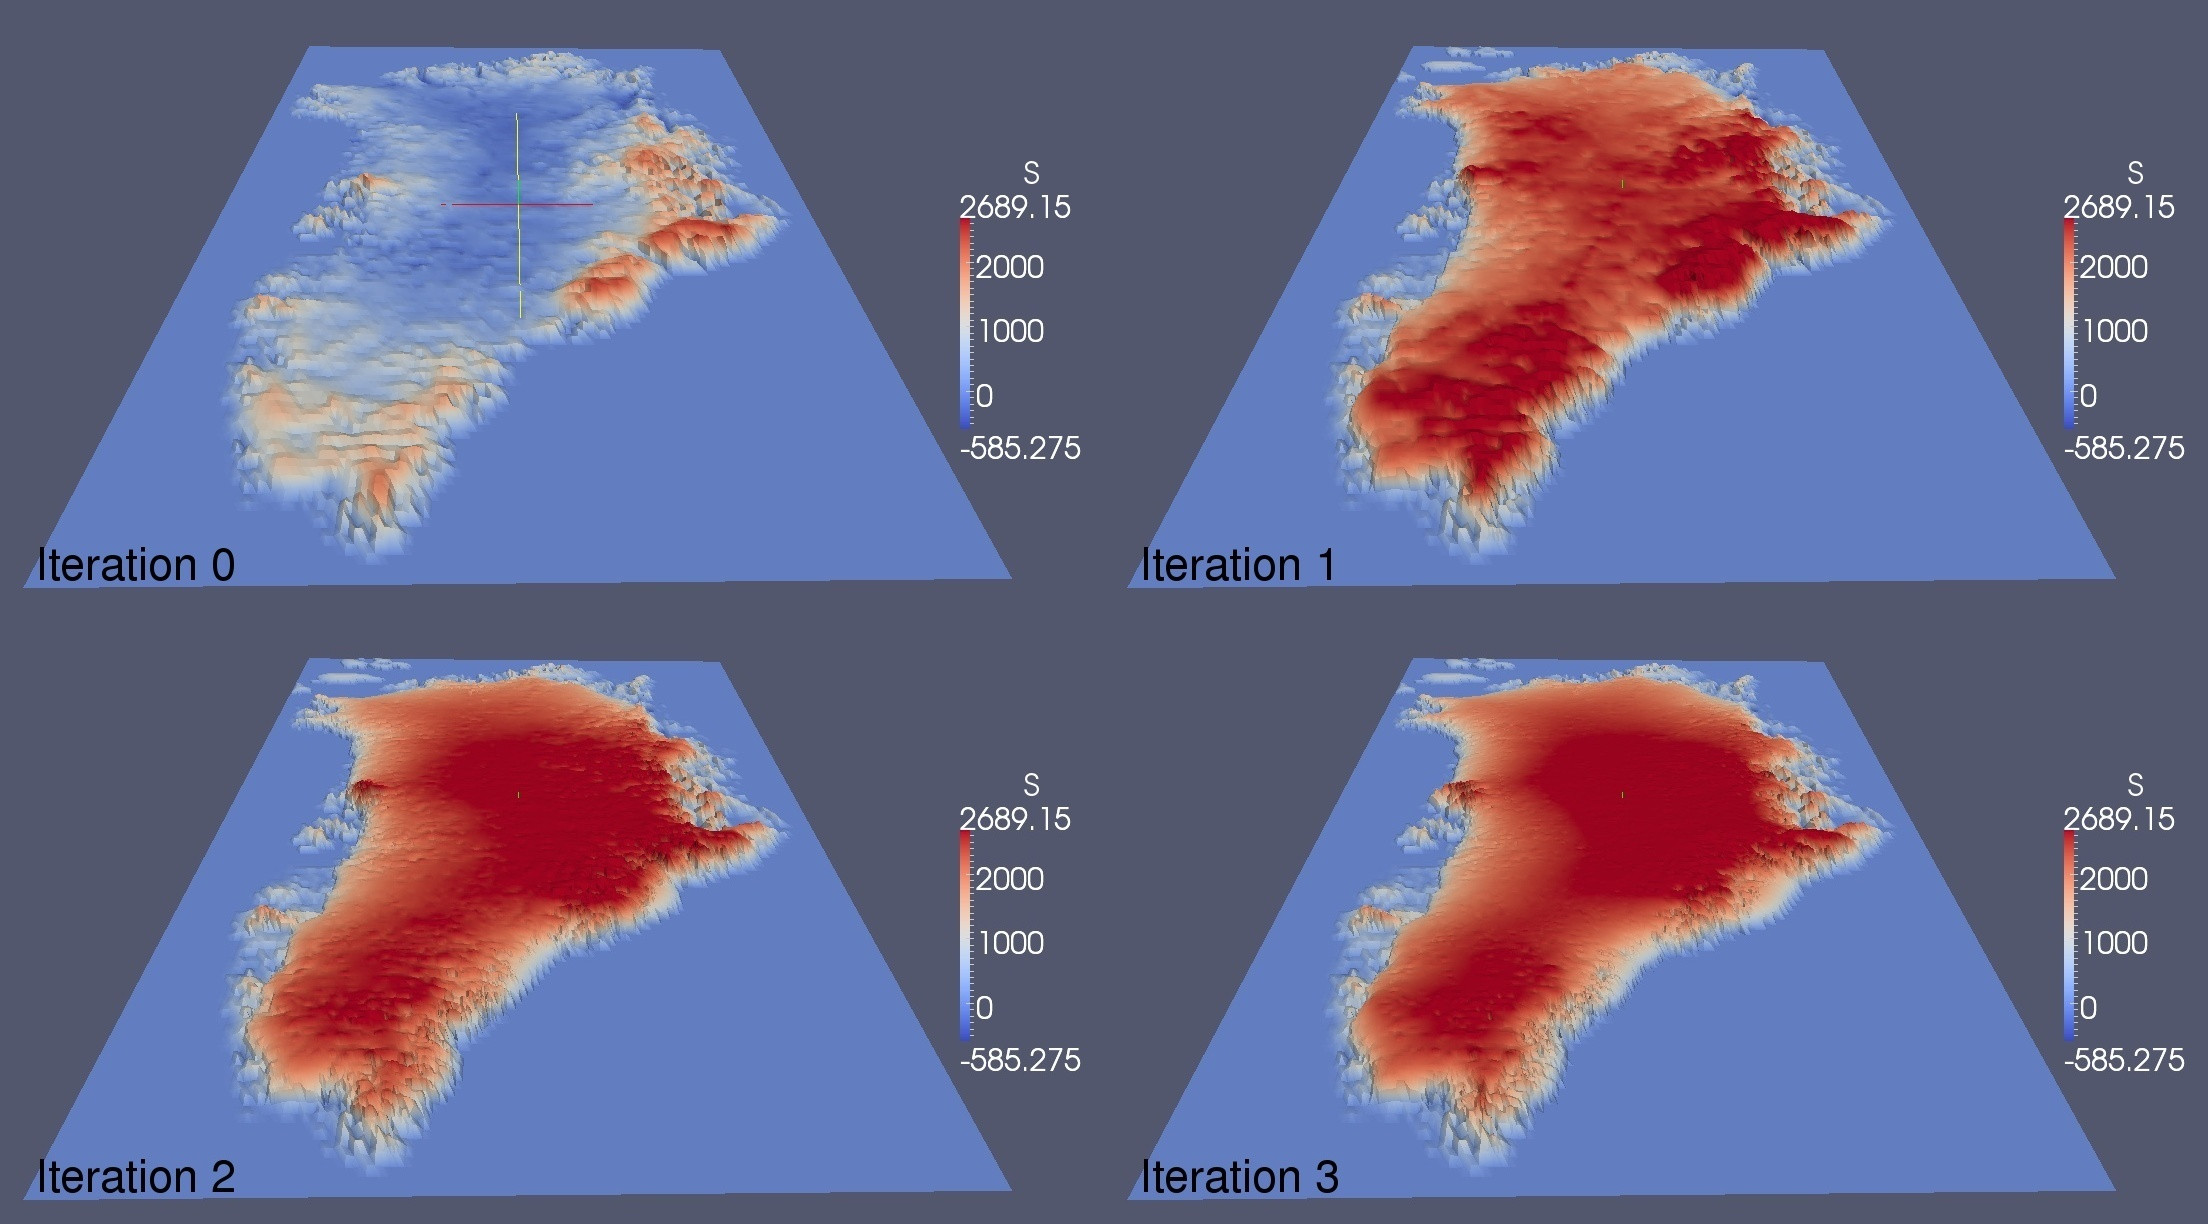
\includegraphics[width=0.9\textwidth]{greenland-result.jpg}
\end{center}
\end{frame}


\section[ice streams]{a model for ice streaming}

\section[marine ice sheets]{a model for marine ice sheet evolution}

\section[polythermal ice]{awaiting a weak formulation: polythermal ice}


\end{document}

